        %%%%%%%%%%%%%%%%%%%%%%%%%%%%%%%%%%%%%%%%%%%%%%%%%%%%%%%%%%%%%%%%%%%%%%%%%%%%%%%%%%%%
%Do not alter this block of commands.  If you're proficient at LaTeX, you may include additional packages, create macros, etc. immediately below this block of commands, but make sure to NOT alter the header, margin, and comment settings here. 
\documentclass[12pt]{article}
 \usepackage[margin=1in]{geometry} 
\usepackage{amsmath,amsthm,amssymb,amsfonts, enumitem, fancyhdr, color, hyperref,comment, graphicx, environ,mathtools, bbm, tikz, setspace, cleveref,listings, dcolumn}
\usepackage{array, multirow, caption, booktabs}
\usepackage{ mathrsfs }
\usetikzlibrary{matrix,positioning}
\tikzset{bullet/.style={circle,draw=black,inner sep=8pt}}
\DeclareMathOperator*{\argmax}{arg\,max}
\DeclareMathOperator*{\argmin}{arg\,min}
\DeclareMathOperator*{\Var}{\text{Var}}
\DeclareMathOperator*{\Cov}{\text{Cov}}

\DeclarePairedDelimiter\norm{\lVert}{\rVert}%
\newtheorem{theorem}{Theorem}
\newtheorem{lemma}[theorem]{Lemma}
\DeclareMathOperator{\eps}{\varepsilon}
\doublespacing
\DeclarePairedDelimiter\abs{\lvert}{\rvert}%
\pagestyle{fancy}
\setlength{\headheight}{65pt}
\newenvironment{problem}[2][Problem]{\begin{trivlist}
\item[\hskip \labelsep {\bfseries #1}\hskip \labelsep {\bfseries #2.}]}{\end{trivlist}}
\newenvironment{sol}
    {\emph{Solution:}
    }
    {
    \qed
    }


%%%%%%%%%%%%%%%%%%%%%%%%%%%%%%%%%%%%%%%%%%%%%%%%%%%%%%%%%%%%%%%%%%%%%%%%%%%%%%%%%


\usepackage{xcolor}
 
 


%%%%%%%%%%%%%%%%%%%%%%%%%%%%%%%%%%%%%%%%%%%%%

\rhead{Asha Bharadwaj, Caitlin Dutta, John Higgins, Alexis Smith\\Econ 899 \\ 29 September, 2022} 

%%%%%%%%%%%%%%%%%%%%%%%%%%%%%%%%%%%%%%%%%%%%%


%%%%%%%%%%%%%%%%%%%%%%%%%%%%%%%%%%%%%%

\begin{document}

\section{I. Solving dynamic programming problem}
The value function over $a$ for a retired agent at model-age 50 is plotted below:
\begin{center}
    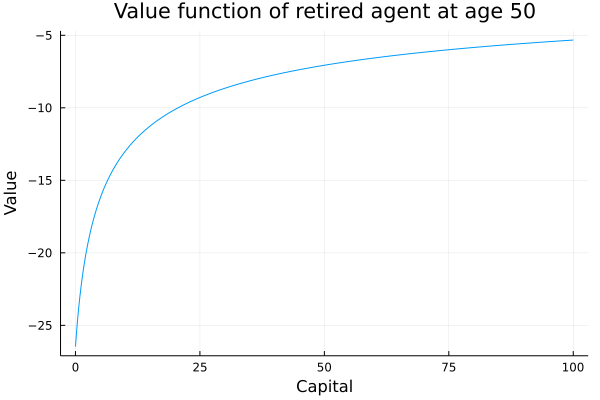
\includegraphics[scale=0.5]{vfplot50.png}
\end{center}
By visual inspection, we can see that it is indeed increasing and concave.

We now look at the savings functions for an agent of model age 20, plotted below along with the labor supply functions:
\begin{center}
    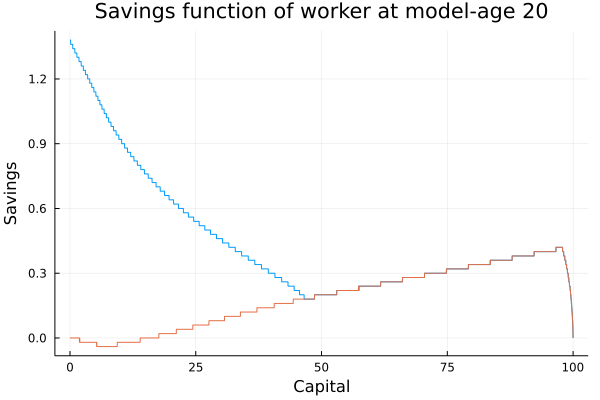
\includegraphics[scale=0.5]{savplot20.png}
\end{center}
\begin{center}
    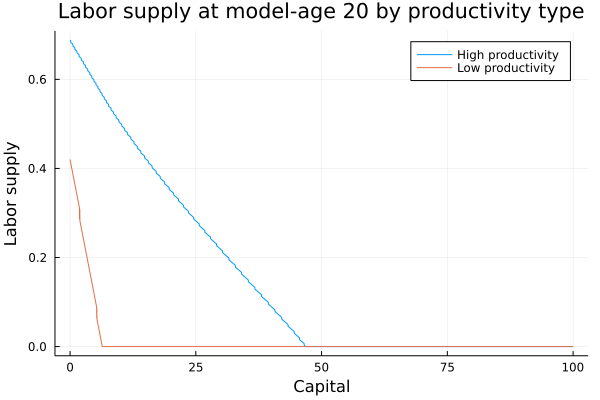
\includegraphics[scale=0.5]{labplot20.png}
\end{center}
We see that the savings function is increasing in $z$. The savings function is generally non-monotone in the level of assets. We can break the relationship down as follows:
\begin{itemize}
 \item High-productivity agents with few assets have the most incentive to save. They have the ability to save a lot due to their high income, and they desire to smooth their consumption in future states. The prospect of transitioning to the low productivity state leads them to accumulate precautionary savings in order to smooth consumption. As their level of assets increases, they are better able to consumption smooth and thus don't have to save quite as much. 
 \item Once high productivity agents have more than $a \approx 50$, however, they start increasing their savings again. It is important to note that at this asset level, high productivity agents choose not to work (this is evident in the labor policy function, included below). They simply live off of the interest of their asset holdings. As the amount of assets they have increases, they consume a smaller proportion of their asset earnings (due to declining marginal utility), which leads to higher savings rates as asset levels increase.
 \item High productivity agents with sufficiently high assets cannot choose a capital level higher than the upper bound on the capital grid. This is the reason why the savings function goes to zero as a reaches the upper bound. This is entirely an artifact of the fact that they are constrained in their choice of capital and has no deep economic meaning.
 \item Low productivity agents with low wealth levels will dissave: their marginal utility of consumption outweighs their expected future marginal utility.
 \item As low productivity agents' asset holdings increase, they have an incentive to save more. This is because they are relatively likely to stay in the low productivity state (as the probability of being in the low state in the next period is over 98\%). This leads them to have high precautionary savings so that they can have higher consumption through the (likely lengthy) bad times ahead. 
\end{itemize}
 \section{II. Economic consequences of eliminating Social Security}
We summarize the results of the policy experiment in the following table. 
\begin{table}[!h]
    \label{Welfare comparisons}
    \begin{center}
    \begin{tabular}{| c | c | c | c | c | c | c |}
    \hline
     & \multicolumn{2}{ c |}{\textbf{Benchmark model}} & \multicolumn{2}{ c |}{\textbf{No risk, $z^L = z^H = 0.5$}} & \multicolumn{2}{ c |}{\textbf{Exog. labor supply, $\gamma = 1$}}  \\ 
    \cline{2-7}
    & \textbf{With SS} & \textbf{w/o SS} & \textbf{With SS} & \textbf{w/o SS} & \textbf{With SS} & \textbf{w/o SS} \\
    \hline
    Capital $K$ &3.360 &4.604 & 1.043& 1.301&7.356 &10.487 \\ \hline
    Labor $L$ & 0.343& 0.365& 0.160&0.169 &0.753 & 0.754\\ \hline
    Wage $w$ & 1.455 & 1.594& 1.256& 1.333&1.454 & 1.651\\ \hline
    Interest $r$ & 0.024& 0.011 & 0.049& 0.038&0.024 & 0.007\\ \hline
    Benefit $b$ & 0.225& 0 & 0.091&0 &0.494 &0 \\ \hline
    Total Welfare $W$ &-35.767 &-37.384 & -45.042& -45.112& -23.008& -25.756 \\ \hline
    CV (wealth) & 1.530& 1.398& 0.6636&0.760& 1.510& 1.329\\ \hline
    \end{tabular}
    \end{center}
    \end{table}

\begin{enumerate}
   \item The benchmark model with social security is dynamically efficient, since the interest rate is 0.024, which exceeds the rate of population growth (i.e. the implicit return from social security). When we eliminate social security, we see that aggregate capital increases and aggregate labor supply increases as well. Capital increases because the elimination of benefits in retirement means that agents need to save more in order to smooth their consumption in retirement. This means that agents increase their savings while they are working so that they have more in retirement, which leads to higher levels of aggregate capital accumulation. Labor supply increases because the removal of a distortionary labor tax leads to an increase in each worker's labor supply. This in turn leads to higher income for agents (which then means they can afford to save more, which feeds into the fact that capital accumulation increases). Aggregate welfare decreases following the policy change since the elimination of the transfer makes the cross-sectional wealth distribution less equal. Older agents will be worse off because of the elimination of the pension benefit. In order to compensate, they must save more when they are working, which trades off with their consumption when young. The young benefit as a result of this policy, since the labor tax is eliminated and they don't have to make transfers to the old. Cross-sectional wealth inequality increases due to the coefficient of variation decreasing (this is the standard deviation of wealth divided by mean wealth): the old become poorer and the young become richer. The mean wealth with social security is 3.944, whereas it is 5.236 after. The standard deviation is 6.027 before, and 7.343 after. So the CV decreases because the mean increases more than the standard deviation. Nevertheless, inequality increases.
   \item We now consider what happens when there is no idiosyncratic risk. We observe that aggregate capital is far lower than in the benchmark model. This is because agents don't have any bad state to insure against; they have no uncertainty and no need to consumption smooth across future (bad) states. They only face an intertemporal tradeoff, where they save in the current stage to smooth consumption across their lifetime. They know the deterministic earnings profile that they face, and they smooth consumption based on that. When we eliminate social security, aggregate welfare decreases. However, the decrease is not nearly as sizeable as the decrease in the benchmark case: the benchmark sees a change of nearly -2, whereas this parameterization has a difference of around -0.5. This suggests that social security plays a role in insuring against idiosyncratic risk: even if an agent is in a low productivity state for most of their life, they are guaranteed $b$ in retirement with social security. In the model without idiosyncratic risk, everyone has the same deterministic earnings profile and thus there may not be as much benefit to social security (as such a system just transfers from workers to those who are old). However, aggregate welfare comparisons can be misleading because they don't account for the distribution of welfare across agents. This means that welfare comparisons must be done carefully and may obfuscate important properties of either equilibrium.
   \item When labor supply is exogenous, we see that labor supply is virtually unchanged due to the elimination of social security. This makes sense, since if labor supply is exogenous and thus inelastic, the labor taxes are not distortionary. Hence, the elimination of social security has no impact on labor supply. To determine who supports this policy, we compute the equivalent variation of consumption for each agent. As in Conesa and Krueger, the EV of an agent of age $n$ with assets $a$ and productivity $z$ is given by
   \[\lambda(n, a,z) = EV_c(n,a,z) = \left( \frac{V_{NSS}(n, a, z)}{V_{SS}(n, a, z)}\right)^{\frac{1}{\gamma(1-\sigma)}}-1\]
   where $V_{NSS}$ is the value function in the equilibrium without social security, and $V_{SS}$ indicates the value function in the equilibrium with social security. We first compute that the total proportion of the population which prefers the elimination of social security is about $16.31\%$. This is the mass of agents with $\lambda(n, a, z) \geq 0$ (i.e., agents who are better off under the new steady state). Furthermore, we plot the proportion of agents within each age which would prefer the elimination of social security below, for both the benchmark model and the one with inelastic labor supply:
   \begin{center}
   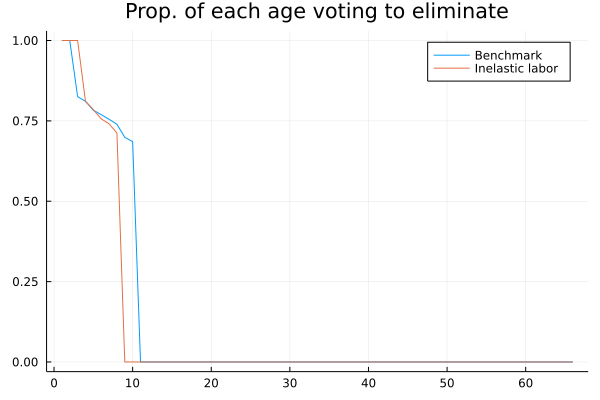
\includegraphics[scale=0.5]{ageplot_in.png}
   \end{center}
   The youngest agents overwhelmingly support the elimination of social security, but the support quickly drops to zero past model-age 10. We see that more agents support elimination in the benchmark model than in the model with inelastic demand. This implies that in the model with inelastic demand, younger agents aren't as adversely affected by social security.
\end{enumerate} 
\end{document}
